\documentclass[a4paper,12pt]{article}

\usepackage[utf8]{inputenc}
\usepackage[T1]{fontenc}
\usepackage{lmodern}
\usepackage[italian]{babel}
\usepackage{float}
\usepackage{graphicx}
\usepackage{subcaption}
\usepackage{amsmath}
\usepackage{amsthm}
\usepackage{amssymb}
\usepackage{xfrac}
\usepackage{url}
\usepackage{listings}
\usepackage{fancyvrb}
\usepackage{multicol}

\setlength{\parskip}{0.5em}

\theoremstyle{definition}
\newtheorem{definition}{Definizione}
\newtheorem{proposition}{Proposizione}

\lstset{ 
	basicstyle=\scriptsize, % the size of the fonts that are used for the code
    language=C,             % the language of the code
    numbers=left,           % where to put the line-numbers (none, left, right)
    tabsize=4,	            % sets default tabsize to 4 spaces
}

\title{Ipotesi di operatore nomadico di reti di sensori}
% \date{2018\\ Dicembre}
% \author{Mattia Dalla Via\\ Dipartimento di Ignegneria dell'Informazione\\ Università degli Studi di Padova}

% quadro, tassello mancante, divario
% rilevanza, apprezzando, opportunità, maturando
% ecosistema
% prestazioni
% rete di transito
% costellazione
% rendezvous

% WSN - Wireless Sensor Network
% MANET - Mobile Ad-hoc Network
% LPWAN - Low Power Wide Area Network

% http://research.protocollabs.com/osm-mobility/

\begin{document}

\maketitle

% \clearpage

\tableofcontents

\section{Introduzione}

Il mercato sta dimostrando un crescente interesse per la raccolta di dati tramite sensori di piccole dimensioni disseminati sul territorio. Questo è possibile mediante l'impiego di dispositivi dotati di moduli radio a basso consumo e a larga portata, tipicamente alimentati a batteria. Inoltre, è necessaria la presenza di concentratori che catturano le trasmissioni e inoltrano i dati al sistema informativo del cliente. L'architettura di queste infrastrutture tende a replicare quella degli operatori di telefonia mobile: è costituita perciò da una serie di concentratori fissi installati sul territorio, connessi in una rete tipicamente cablata. Tale soluzione, seppur molto affidabile, richiede un grande investimento iniziale e presenta dei tempi di messa in opera tendenzialmente lunghi. Esistono allo studio altre tipologie di rete, dette ad hoc, che non prevedono un'infrastruttura. Queste si basano sulla capacità dei dispositivi di inoltrare le informazioni, per costituire essi stessi una dorsale indipendente priva di un collettore. In quest'ottica, esploreremo un paradigma alternativo che prevede la raccolta best effort di informazione da sensori fissi o mobili sparsi nel territorio, da parte di concentratori che anziché essere fissi sono in movimento. Lo scenario prevede un operatore che chiameremo nomadico che impega un'infrastruttura di raccolta dati montata su veicoli.

% In questa tesi esploreremo un paradigma alternativo con l'obiettivo di offrire una copertura estesa e flessibile, immediatamente disponibile ad un costo inferiore.

% Molte imprese di telecomunicazioni si stanno quindi adoperando per offrire soluzioni di connettività mediante la realizzazione di infrastrutture geografiche.

% Per rispondere al crescente interesse nei confronti dell'IoT, una nuova categoria di tecnologie di comunicazione wireless sta emergendo. Reti di sensori o oggetti autonomi pongono nuovi vincoli e necessità rispetto ai classici approcci di connettività. Al contempo, alcuni aspetti ritenuti classicamnete cruciali nella valutazione di una rete, assumono un'importanza secondaria e lasciano quindi spazio a nuovi modelli di funzionamento.

% La caratteristica che accomuna la grande maggioranza delle soluzioni IoT è la limitata disponibilità di energia: questi dispositivi sono infatti normalmente alimentati a batteria. Le principali soluzioni di connettività orbitano quindi attorno a questa recessità, focalizzandosi sul limitare i tempi di attività di trasmissione e ricezione.

\section{Architetture di rete}

In questa sezione descriveremo innanzitutto l'architettura di LoRa, come esempio di organizzazione classica di una rete di sensori. Proseguiremo poi con la proposta di un modello che si promette come valida alternativa in uno spettro di applicazioni dove le soluzioni classiche risultano poco pratiche o eccessivamente costose.

\subsection{LoRa}

LoRa è una tecnologia di comunicazione wireless punto-punto che utilizza una modulazione a spettro espanso. È pensata per applicazioni embedded, sacrificando la banda per offre una copertura a lungo raggio (più di 10km in zone rurali) con un consumo minimo di energia \cite{loraperf}. LoRaWAN è un protocollo MAC basato sul livello fisico LoRa promosso da LoRa Alliance. Esso funge da protocollo di rete, definendone l'architettura e gestendo le comunicazioni tra gateway e nodi. La loro combinazione offre una soluzione completa, adottata da molti fornitori di servizi di connettività \cite{netprov}.

Una rete LoRaWAN si compone di quattro classi di oggetti \cite{loraspec}:

\begin{enumerate}
\item End nodes: i sensori, dotati di modulo radio LoRa.
\item Gateway: stazioni radio base, ricevono le trasmissioni dei sensori.
\item Network Server: connesso ai gateway, smista il traffico di dati ricevuto inoltrandolo ai relativi server dei clienti.
\item Application Server: parte del sistema informativo del cliente, consuma i dati raccolti.
\end{enumerate}

\begin{figure}[H]
\centering
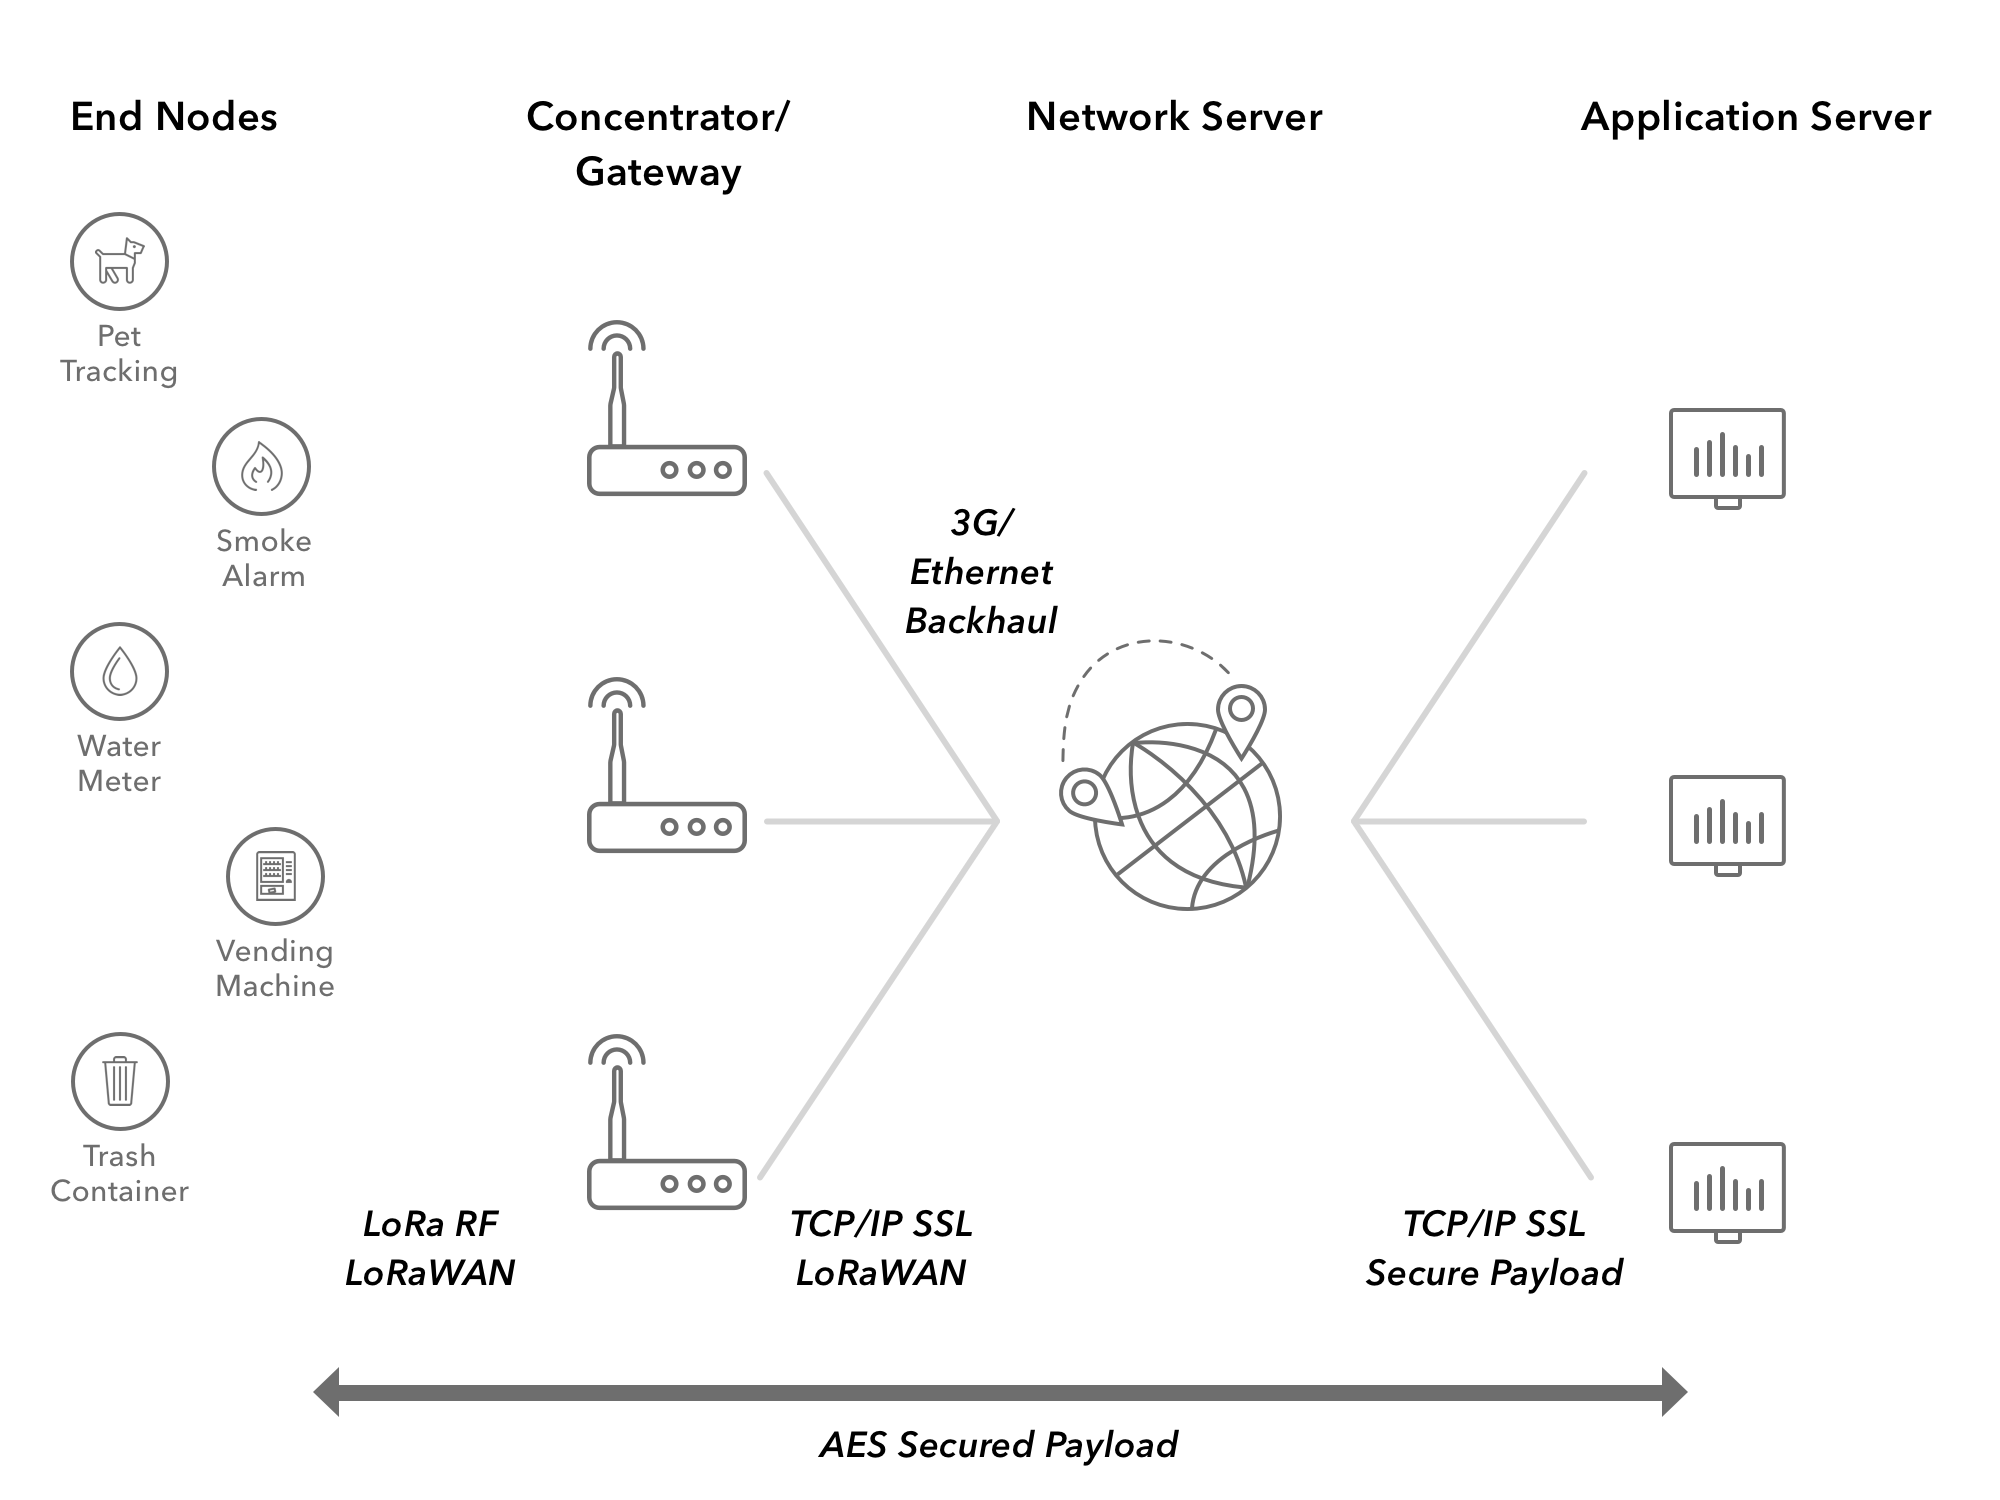
\includegraphics[width=10cm]{figures/lorawan.png}
\caption{Architettura di una rete LoRaWAN.}
\end{figure}

% https://www.thethingsnetwork.org/docs/lorawan/LoRaWAN-Overview.png

Gli operatori forniscono perciò il proprio servizio installando sul territorio dei gateway, connessi al proprio network server. Questi sono tipicamente situati in punti strategici, dotati di alimentazione e connessione ad Internet. La topologia è a stella: le trasmissioni dei nodi vengono ricevute esclusivemente da uno o più gateway \cite{loraspec}. La copertura è perciò dettata dalla presenza degli stessi, richiedendo eventualmente nuove installazioni per essere estesa.

\subsection{Rete ad hoc}

\subsection{Infrastruttura nomadica}

In alternativa alla collocazione statica dei gateway esiste l'idea, nota in letteratura come \emph{sink mobility}, di un'infrastruttura mobile che cambia posizione all'interno del territorio \cite{sinkmob}. Immaginiamo di seguito un operatore che raccoglie dati dai sensori mediante stazioni radio base installate su veicoli in movimento. Per estendere la copertura oltre la cella mobile, adottiamo un instadamento multi-hop: Qualora necessario, il messaggio viene ritrasmesso dai nodi della rete fino alla destinazione.

\begin{figure}[H]
\centering
\includegraphics{figures/nomadic.pdf}
\caption{Sink mobile che raccoglie dati dai sensori.}
\end{figure}

L'utilizzo di sink mobile è generalmente motivato dalla seguente osservazione di carattere energetico: In una rete di sensori ad-hoc, la concentrazione del traffico nelle vicinaze dei sink fa si che le batterie dei nodi si eusauriscano in maniera disomogenea. Riposizionare periodicamente i sink diventa perciò una semplice strategia per bilanciare i livelli di carica dei sensori \cite{moblife1, moblife2}.

Un altro aspetto, meno popolare in letteratura ma a nostro avviso estremamente rilevante è il seguente: La frequenza di raccolta dati dai sensori è, in generale, piuttosto bassa. In molte applicazioni si limita ad esempio a non più di un aggiornamento al giorno. La presenza di un'infrastruttura statica disponibile in ogni momento risulta per questo motivo superflua. Essa è sostituibile, come precedentemente anticipato, da veicoli di raccolta dati che transitano con sufficiente frequenza in prossimità dei sensori. Una simile strategia richiede non solo un numero più limitato di sink a parità di territorio, ma permette di offrire copertura in tempi rapidi. Tale copertura può essere inoltre rilocata o redistribuita nel tempo senza la necessità di nuove installazioni.

Per questi motivi riteniamo che un'infrastruttura nomadica costituisca, nelle giuste condizioni, un'alternativa economica e flessibile alle soluzioni classiche. Alla luce di ciò, proseguiremo in questo elaborato fornendo dapprima una descrizione formale del problema, proseguendo poi con una sua analisi e con la proposta di un algoritmo di instradamento confacente.

\section{Modello}

Cosa intendiamo esattamente quando facciamo riferimento ad una rete di sensori? In questa sezione proponiamo un modello che ne schematizza le caratteristiche fondamentali.

% Questo modello non ha lo scopo di rappresentare una rete in generale, bensì è calzato su misura per semplificare la descrizione dell'algoritmo.

% \subsection{Nodi e ambiente}

Consideriamo una rete composta da $n+1$ nodi, ciascuno identificato da un indice $i \in \{0, \dots, n\}$ univoco. Il nodo di indice $i=0$, detto \emph{sink}, costituisce il destinatario finale di tutti i messaggi e svolge il ruolo di gateway verso il sistema informativo sovrastante. Tutti gli altri nodi, chiamati satelliti, sono i veri e propri sensori.

Chiamiamo \emph{portata} (del segnale) la distanza massima $p$ a cui è possibile trasmettere dati e supponiamo sia uguale per tutti i nodi. Inoltre, definiamo una regione di spazio \emph{ambiente} di raggio $a$ centrato nel sink, nel quale sono distribuiti i satelliti.

\begin{figure}[H]
\centering
\includegraphics{figures/model.pdf}
\caption{Rete di 4 satelliti, di cui 3 connessi al sink.}
\end{figure}

Questa descrizione trascura la dimensione temporale e di conseguenza gli spostamenti relativi dei nodi. Ipotizziamo infatti che la magnitudine dei movimenti nel lasso di tempo delle comunicazioni sia trascurabile rispetto alla portata.

\subsection{Layout di rete}

Con \emph{layout di rete} ci riferiamo ad una specifica configurazione spaziale di $n$ satelliti con portata $p$ in un ambiente di raggio $a$. Parliamo quindi della ``fotografia'' di una rete che ritrae le coordinate di ciascun nodo, la loro portata e l'ampiezza dell'ambiente in cui sono disposti. Ne diamo una definizione formale:

\begin{definition}
Sia
\begin{equation*}
N = \{(0,\,0,\,0),\,(1,\,x_1,\,y_1),\,\dots,\,(i,\,x_i,\,y_i),\,\dots,\,(n,\,x_n,\,y_n)\}
\end{equation*}
un insieme di $n+1$ nodi, di indice $i$ e coordinate $x_i,\,y_i$. Chiamiamo \emph{layout di rete} la tripla
\begin{equation*}
L = (a,\,p,\,N)
\end{equation*}
dove $a$ è il raggio dell'ambiente e $p$ la portata dei nodi.
\end{definition}

Da notare che il sink ($i=0$) ha sempre coordinate $0,\,0$. Mentre per tutti i nodi vale che $dist(0,\,i) = \sqrt{x_i^2+y_i^2} \leq a$.

Vincolando i parametri $a$, $p$ e $n$ otteniamo un sottoinsieme di layout dove solo le coordinate dei satelliti rimangono indeterminate. Chiamiamo questo sottoinsieme $layout(a,\,p,\,n)$. Nelle prossime sezioni esamineremo le relazioni che legano queste variabili e tenteremo di caratterizzare i sottoinsiemi che vanno a produrre. In altre parole ci chiederemo: Fissati $a$, $p$ e $n$, cosa possiamo dire in generale sul layout?

\subsection{Grafo di connettività}

Noto un layout di rete $L$, da esso estrapoliamo un grafo. Questo descrive la connettività della rete, tenendo conto delle relazioni tra i nodi connessi tralasciando le loro posizioni.

\begin{figure}[H]
\centering
\includegraphics{figures/graph.pdf}
\caption{Esempio di grafo di connettività.}
\end{figure}

Questo tipo di descrizione della rete si avvicina di più a quella a disposizione degli algoritmi di routing. Le coordinate dei nodi sono spesso infatti ignote, mentre le distanze sono stimabili sulla base della potenza del segnale ricevuto. Diamo anche per il grafo una definizione formale:

\begin{definition}
Siano $V = \{0,\,\dots,\,n\}$ gli indici di $n+1$ nodi con portata $p$. Siano $E$ gli archi (connessioni) tra i nodi, calcolati come:
\begin{equation*}
E = \{ (i,\,j) \text{ dove } i,\,j \in V \mid dist(i,\,j) \le p \ \wedge \ i \neq j\}
\end{equation*}
chiamiamo $G = (V,\,E)$ il \emph{grafo di connettività}.
\end{definition}

% E = \{ (i,\,j,\,w) \text{ dove } i,\,j \in V \text{ e } w = \frac{dist(i,\,j)}{p} \mid w \le 1 \ \wedge \ i \neq j\}

La funzione $dist(i,\,j)$ rappresenta la distanza tra la coppia di nodi. Nelle successive simulazioni sarà definita come la distanza geometrica tra le coordinate.

% Nel caso queste non siano note, la distanza potrebbe essere valutata grazie alla potenza di ricezione dei messaggi.

Diremo che $G = graph(L)$ è il grafo associato al layout $L$ se questo è calcolato sulle coordinate dei nodi di $L$ e sulla loro portata. Chiamiamo \emph{sottografo connesso} $C \subseteq G$ il sottografo contenente il sink e diremo \emph{connessi al sink} tutti i nodo in esso contenuti, ovvero tutti quelli che hanno almeno un cammino che li collega al sink. Se $G = C$ diremo che $G$ è \emph{completamente connesso}.

Al contrario di quanto si potrebbe pensare, il passaggio per il concetto di layout non risulta affatto superfluo. Basando la propria rappresentazione direttamente su di un grafo si rischia infatti di descrivere situazioni che non rispettano i vincoli geometrici del piano. Ad esempio: noto che $dist(i,\,j) = dist(j,\,k) = 1$, allora necessariamente $0 \leq dist(i,\,k) \leq 2$. In altri termini possiamo dire che la funzione $graph(L)$ non è suriettiva. Alla luce di questo, chiamiamo \emph{realistico} un grafo a cui è associato almeno un layout.

Dato un grafo realistico $G$, esistono in realtà infiniti layout \emph{topologicamente equivalenti} tali che $G = graph(L_i)$ che vengono mappati sullo stesso grafo. In altre parole $graph(L)$ non è iniettiva. In particolare, dato
\begin{equation*}
L = (a,\,p,\,\{(0,\,0,\,0),\,(1,\,x_1,\,y_1),\,\dots,\,(i,\,x_i,\,y_i),\,\dots,\,(n,\,x_n,\,y_n)\})
\end{equation*}
chiamiamo \emph{layout in scala} $m$ il layout
\begin{equation*}
scale(L,\,m) = (a\,\cdot\,m,\,p\,\cdot\,m,\,\{(0,\,0,\,0),\,\dots,\,(i,\,x_i\,\cdot\,m,\,y_i\,\cdot\,m),\,\dots\})
\end{equation*}
con $m \in \mathbb{Q}_{>0}$. I layout in scala sono tutti topologicamente equivalenti poiché
\begin{equation*}
\frac{dist(i_m,\,j_m)}{p_m} = \frac{dist(i,\,j)\,\cdot\,m}{p\,\cdot\,m} = \frac{dist(i,\,j)}{p}	
\end{equation*}
ovvero le distanze relative si conservano. Consideriamo ad esempio
\begin{align*}
L_5 = (10,\,5,\,\{(0,\,0,\,0),\,(1,\,4,\,1),\,(2,\,-2,\,-3)\})\\
L_{15} = (30,\,15,\,\{(0,\,0,\,0),\,(1,\,12,\,3),\,(2,\,-6,\,-9)\})
\end{align*}
questi layout sono topologicamente equivalenti, in particolare $L_{15} = scale(L_5,\,3)$. Entrambi vengono perciò mappati nello stesso grafo
\begin{equation*}
graph(L_5) = graph(L_{15}) = (\{0,\,1,\,2\},\,\{(0,\,1),\,(0,\,2),\,(1,\,0),\,(2,\,0)\})
\end{equation*}
Ci rendiamo quindi conto che sarà sufficiente studiare il sottoinsieme $layout(a,\,1,\,n)$ poiché qualsiasi layout $L_u$ con $p=u \in \mathbb{Q}_{>0}$ sarà equivalente a $L_1 = scale(L_u,\,\frac{1}{u})$. Ovvero $layout(a,\,p,\,n)$ è equivalente a $layout(\frac{a}{p},\,1,\,n)$.

\subsection{Dimensione e densità}

% relazioni caratteristiche

% Appare subito evidente che la portata e il raggio dell'ambiente influenzano in maniera interdipendente il modello. In particolare, fissati $r_0$ e $p_0$, è possibile definire una classe di reti dove $r = m \cdot r_0, \ p = m \cdot p_0$ con $m \in \mathbb{Q}_{>0}$ e dove le posizioni relative dei nodi sono conservate. Queste reti sono equivalenti a meno di un fattore di scala. È utile quindi definire il concetto di \emph{guadagno}, per identificare tutte quelle reti appartenenti a classi distinte.

Alla luce di quanto appreso nella sezione precedente, introduciamo ora il concetto di \emph{dimensione del layout}. Questo esprime il raggio ambiente utilizzando la portata come unità di misura. In altre parole potremmo dire che è il raggio ambiente normalizzato su $p$.

\begin{definition}
Sia $a$ il raggio ambiente e $p$ la portata dei nodi. La \emph{dimensione radiale} $d$ è il loro rapporto:
\begin{equation*}
d = \frac{a}{p}
\end{equation*}
\end{definition}

\begin{definition}
Sia $a$ il raggio ambiente e $p$ la portata dei nodi. La \emph{dimensione superficiale} $D$ è il rapporto tra l'area coperta da un singolo nodo e l'area totale dell'ambiente:
\begin{equation*}
D = \frac{\pi a^2}{\pi p^2} = \left(\frac{a}{p}\right)^2 = d^2
\end{equation*}
\end{definition}

Nell'ottica dei layout in scala, dato $L_p = (a,\,p,\,N)$, possiamo dire che $d$ è il raggio ambiente del layout equivalente $L_1 = (d,\,1,\,N)$. Come menzionato in precedenza sarà perciò sufficiente studiare i layout al variare di $d$ ($layout(d,\,1,\,n)$) per coprire l'intero spazio dei grafi di rete.

% Queste definizioni rispondono alla seguente domanda: Fissata la portata dei nodi, quanto è più grande l'ambiente in cui sono disposti? In pratica queste grandezze normalizzano le misure di lunghezza e superficie, usando $p$ come unità di misura.

Definiamo infine una speciale relazione tra $n$ e $d$ che sarà di centrale importanza per l'analisi delle proprietà di $L$:

\begin{definition}
Sia $n$ il numero di satelliti e $d$ la dimensione radiale, chiamiamo \emph{densità di nodi} $q$ la relazione:
\begin{equation*}
q = \frac{n}{d^2} = \frac{n}{D}
\end{equation*}
\end{definition}

Questo rapporto ci da un'informazione sulla quantità di nodi per unità di superificie.

\subsection{Tempo}

Ipotizziamo che i nodi siano dotati di un orologio sincronizzato e siano perciò in grado di accendersi contemporaneamente e operare in modo coordinato. Per semplicità misureremo il tempo in modo che la durata di una trasmissione coincida con un quanto temporale. Una trasmissione iniziata a $t$ terminerà quindi entro $t+1$. Per il resto della tesi ci riferiremo a $t=0$ come l'istante iniziale di accensione della rete e a $t$ come l'istante corrente.

\begin{figure}[H]
\centering
\includegraphics{figures/time.pdf}
\caption{Schema della suddivisione temporale.}
\end{figure}

Il tempo è suddiviso in \emph{frame} della durata di 3 quanti temporali. Chiamiamo $frame(t) =  \left\lfloor\frac{t}{3}\right\rfloor$ il frame associato all'istante $t$. Ciascun frame è suddiviso in 3 \emph{slot}, indicizzati $0,\,1 \text{ e } 2$. Chiamiamo $slot(t) = t \bmod 3$ lo slot associato all'istante $t$. Questa suddivisione sarà in seguito giustificata come multiplazione temporale, parte del meccanismo di prevenzione delle collisioni.

\subsection{Canale}

Il \emph{canale} è un numero naturale. Esso costituisce un'astrazione per il multiplexing di frequenza o un qualsiasi altro meccanismo di multiplazione che permetta a due moduli radio di trasmettere contemporaneamente senza interferenze.

Ipotizziamo che all'istante $t$ stiano trasmettendo i due nodi $i$ e $j$: se $k$ è connesso ad entrambi ($dist(k,\,i) \leq p,\,dist(k,\,j) \leq p$) e se le trasmissioni avvengono sullo stesso canale ($channel(i) = channel(j)$) parliamo di \emph{collisione} in $k$. Da notare che, trattandosi di comunicazione radio, due o più trasmissioni contemporanee sullo stesso canale non necessariamente collidono in tutti i punti dello spazio.

\begin{figure}[H]
\centering
\includegraphics{figures/collision.pdf}
\caption{Regione di interferenza.}
\end{figure}

In questo esempio, $i$ e $j$ stanno trasmettendo. $k$ si trova nella \emph{regione di interferenza} e perciò non riceverà il messaggio. $q$ invece è raggiunto solamente dal segnale di $j$ e perciò non soffrirà dell'interferenza.

% modello radio

\section{Analisi}

Muniti di una descrizione formale di rete, rappresentata dal layout $L = (a,\,p,\,N)$ e dal relativo grafo $G = graph(L)$, andiamo ora ad analizzare le sue caratteristiche al variare di $a$, $p$ e $n$. In questa sezione proponiamo due possibili disposizioni dei satelliti nell'ambiente, studiando la connettività dei grafi associati.

\subsection{Rapporto di connessione}

Individuiamo innanzitutto una metrica con la quale valutare $G$:

\begin{definition}
Sia $R$ l'insieme dei possibili grafi di rete. Chiamiamo \emph{rapporto di connessione} la funzione
\begin{equation*}
c \colon R \to [0,\,1]
\end{equation*}
che mappa $G$ nel numero relativo (percentuale) di satelliti connessi al sink.
\end{definition}

Questa risponde alla domanda: dato un grafo $G \in R$, quanti dei satelliti risultano connessi al nodo sink? Dà quindi un'informazione sulla quantità dei nodi nel sottografo connesso.

Quanto vale il rapporto di connessione al variare dei parametri $a$, $p$ e $n$? Questa domanda non trova una risposta generale, in quanto esso fondamentalmente dipende dallo specifico grafo di rete. Banalmente, se fissiamo $d = 1$, la porata del sink coprirà l'intero ambiente e perciò tutti i satelliti saranno ad esso direttamente connessi, ovvero $c(G) = 1 \ \forall G = graph(L)$ con $d = 1$. Posto invece $d > 1$, tutti i satelliti potrebbero rientrare nella portata del sink e quindi risultare $c(G_1) = 1$, oppure viceversa potrebbero essere tutti a distanza $> p$ dal sink e perciò risultare $c(G_2) = 0$.

\subsection{Layout a reticolo uniforme}

Ipotizzando che i nodi siano disposti in una griglia uniforme, possiamo determinare la soglia per un grafo completamente connesso. Chiamiamo i layout con questa caratteristica \emph{layout a reticolo uniforme} $L_r$ e di conseguenza $G_r = graph(L_r)$.

\begin{figure}[H]
\centering
\includegraphics{figures/layout_ret.pdf}
\caption{Layout a reticolo uniforme.}
\end{figure}

\begin{proposition}
Sia $L_r = (a,\,p,\,N)$ un layout a reticolo uniforme. Sia $G_r = graph(L_r)$ il suo grafo associato. Allora
\begin{equation*}
c(G_r) = 1 \ \text{se e solo se} \ n \geq \frac{4}{\pi} \left(\frac{2a}{p}\right)^2 = \frac{16}{\pi} D
\end{equation*}
dove $D = d^2 = \left(\frac{a}{p}\right)^2$ è la dimensione superficiale.
\end{proposition}

Usando la definizione di densità di nodi: il grafo è completamente connesso quando $q \geq \frac{16}{\pi} \simeq 5.09$.

Questo risultato si ottiene considerando la porzione di area del cerchio di raggio $d = \frac{a}{p}$ inscritto nel quadrato di lato $2d = \frac{2a}{p}$. La proporzione tra l'area del quadrato e del cerchio inscritto è costante a $\frac{4}{\pi}$ mentre l'area del quadrato vale $(2d)^2 = 4D$. La disuguaglianza assicura infine che la distanza tra ogni coppia di nodi in asse sia $\leq p$.

Si ha quindi che con un layout $L_r$, per garantire che tutti i satelliti siano connessi al sink, la coppia $n$, $d$ va scelta secondo la relazione $n \geq \frac{16}{\pi} d^2$.

\begin{figure}[H]
\centering
\includegraphics{figures/ret_locus.pdf}
\caption{Luogo delle coppie $n$, $d$ per le quali $c(G_r) = 1$}
\end{figure}

\subsection{Layout stocastico}

Per studiare il comportamento medio di un campione eterogeneo di layout, ne generiamo automaticamente in funzione di $n$, $a$ e $p$, scengliendo casualmente le coordinate dei satelliti. Questa operazione equivale ad estrarre in maniera aleatoria un elemento dal sottoinsieme $layout(a, p, n)$.

I dati vengono prodotti mediante delle routine scritte in linguaggio C che andiamo ora a dimostrare attraverso l'uso di alcuni esempi:

\texttt{\textbf{layout n a p ----seed s}} genera un layout $L = (a,\,p,\,N)$ con $|N| = n+1$. Le coordinate dei satelliti sono estratte da una fonte di numeri pseudo-casuali inizializzata con il seme $s$. Produce un output nella forma:

\begin{figure}[H]
\centering
\begin{BVerbatim}
n    a    p    s
0    0
x1   y1
x2   y2
 ...
xn   yn
\end{BVerbatim}
\end{figure}

Eseguendo ad esempio \texttt{layout 4 8 5 ----seed 16} otteniamo:

\begin{figure}[H]
\centering
\begin{BVerbatim}
 4    8    5    16
 0    0
 3    2
-4   -3
 8    0
-1   -4
\end{BVerbatim}
\end{figure}

\texttt{\textbf{graph}} legge in input un layout $L$ e ne calcola il relativo grafo. Produce un output nella forma:

\begin{figure}[H]
\centering
\begin{BVerbatim}
n    a    p    c
0    g11  g12  ...  g1n
g11  0    g21  ...  g2n
 ...
gn1  gn2  gn3  ...  0
\end{BVerbatim}
\end{figure}

Il grafo è codificato mediante una matrice: il valore $g_{ij}$ esprime la distanza normalizzata su $p$ tra i nodi $i$ e $j$. Se $g_{ij} \leq 1$ è perciò presente un arco tra la coppia di nodi. $c$ è il numero di satelliti connessi al sink.

Per calcolare il grafo $G$ associato al layout dell'esempio precendete eseguiamo \texttt{layout 4 8 5 ----seed 16 | graph}:

\begin{figure}[H]
\centering
\begin{BVerbatim}
4     8     5     3
0.00  0.72  1.00  1.60  0.82 
0.72  0.00  1.72  1.08  1.44 
1.00  1.72  0.00  2.47  0.63 
1.60  1.08  2.47  0.00  1.97 
0.82  1.44  0.63  1.97  0.00 
\end{BVerbatim}
\end{figure}

Il grafo ottenuto ha un rapporto di connessione $c(G) = \frac{3}{4} = 0.75$.

% Per la creazione di un dataset al variare di $n$ e $d$ utilizzaimo infine

\texttt{\textbf{conn n\_min n\_max n\_step d\_min d\_max d\_step p i ----seed s}} calcola il rapporto di connessione medio tra $i$ campioni per ciascun valore di $n \in \{n_{min},\,n_{min}+n_{step},\,\dots,\,n_{max}\}$ e $d \in \{d_{min},\,d_{min}+d_{step},\,\dots,\,d_{max}\}$. La fonte di numeri pseudo-casuali viene inizializzata a partire dal seme $s$, che viene incrementato per ciascun campione. Produce tre colonne con i valori rispettivamente di $d$, $n$ e $c$.

% \subsection{Rapporto di connessione medio}

Prendiamo ora in esame un dataset\footnote{Disponibile all'indirizzo \url{https://raw.githubusercontent.com/mattiadallavia/adhociot/master/conn.dat}.} generato mediante le routine appena descritte, con l'obiettivo di stimare il \emph{rapporto di connessione medio} $\tilde{c}(q)$ in funzione della densità di nodi. Sottolineiamo che questa non fornirà un'informazione su quali probabilmente saranno i valori di $c(G)$, ma bensì su quali valori medi ci aspettiamo da un grande numero di layout eterogenei.

Il dataset è frutto dell'esecuzione di \texttt{conn 0 1000 50 0 20 1 1000 100 ----seed 1}. Sono stati perciò calcolati 100 campioni per ogni valore di $n \in \{0,\,50,\,100,\,150,\,\dots,\,1000\}$ e $d \in \{0,\,1,\,2,\,\dots,\,20\}$ per un totale di $100 \cdot 20 \cdot 20 = 40\,000$ esperimenti aleatori.

\begin{figure}[H]
\begin{subfigure}[b]{0.5\textwidth}
\includegraphics[width=\textwidth]{figures/conn_3d.pdf}
\end{subfigure}
\begin{subfigure}[b]{0.5\textwidth}
\includegraphics[width=\textwidth]{figures/conn_dim.pdf}
\end{subfigure}
\caption{Visualizzazione del dataset.}
\end{figure}

Come ci si poteva aspettare, al crescere di $d$ il rapporto di connessione medio cala repentinamente: nello specifico, è inversamente proporzionale alla dimensione superficiale $D = d^2$. Questa tendenza è tuttavia mitigata al crescere di $n$, infatti all'aumentare dei satelliti sale la probabilità che si formino dei percorsi al sink.

Interpolando i dati sulla funzione $\tilde{c}(q) = s \cdot tanh(w \cdot q + t) + u$ (determinata empiricamente) otteniamo:
\begin{equation*}
\tilde{c}(q) = 0.5 \cdot tanh(0.97 \cdot q - 4.38) + 0.5
\end{equation*}
dove $q$ è la densità di nodi $q = \frac{n}{D}$.

\begin{figure}[H]
\centering
\includegraphics{figures/conn_den.pdf}
\caption{Grafico di $\tilde{c}(q)$ a confronto con i dati sperimentali.}
\end{figure}

Da questo grafico si evince che un rapporto di connessione medio $\tilde{c} \geq 0.9$ si ottiene quando $d \gtrsim 5.6$. Un risultato del tutto in linea con quello ottenuto per i layout a reticolo uniforme.

\section{Algoritmo}

% instradamento
% complessità
% efficienza
% ciclo di vita
% collisioni / contesa / exponential backoff
% gestione di canale
% formato del messaggio
% Minimizzare le trasmissioni
% Configurare la rete in assenza di un coordinamento prestabilito
% Semplicità della routine di nodo

In questa sezione presentiamo un algoritmo di routing per la raccolta dati dai sensori. La modalità di funzionamento è di tipo ad-hoc: il messaggio viene ritrasmesso dai satelliti lungo un percorso che lo porta al sink. A causa delle possibili interferenze, è necessario l'invio di riscontri per confermare la corretta ricezione dei messaggi. Tuttavia, grazie ad un'attenta schedulazione, gli acknowledgment avvengono nella maggior parte dei casi in piggyback. L'obiettivo è infatti quello di minimizzare le trasmissioni, in quanto queste richiedono il massimo dispendio di energia da parte dei moduli radio. Un'altro fattore importante è quello temporale: è di naturale interesse raccogliere i dati nel minor tempo possibile. Alla luce di questo, scegliamo il numero totale di trasmissioni $tx$ e l'istante di ricezione dell'ultimo messaggio $t_f$ come metriche di valutazione dell'algoritmo.

Ipotizzando che non avvengano collisioni, $n$ messaggi (uno per satellite) vengono consegnati in
\begin{equation*}
tx = \sum_{i=1}^{n} depth(i) + n + 1
\end{equation*}
trasmissioni. Questo si ottiene conteggiando il messaggio iniziale di esplorazione del sink e $depth(i) + 1$ trasmissioni per ciascun messaggio. Nella sezione \ref{simulazione} ricaveremo dei valori medi di $tx$ e $t_f$ su un campione di layout stocastici.

\subsection{Principio di funzionamento}

L'algoritmo opera a macchia d'olio: a $t=0$ il sink da inizio alle trasmissioni con un messaggio di esplorazione. Gli invii a questo punto avvengono a partire dal centro verso la perifieria, procedento man mano in anelli concentrici. Durante questo processo il grafo di rete viene esplorato, determinando concettualmente un albero che collega ciascun satellite al sink ed assegnando ad ogni nodo la propria profondità.

\begin{figure}[H]
\centering
\includegraphics{figures/depths.pdf}
\caption{Esempio di rete con relative profondità.}
\end{figure}

Ogni trasmissione assume una duplice valenza: consideriamo l'invio del messaggio $m$ da parte del nodo $i$ di profondità $p$, questa corrisponde all'inoltro del dato verso i nodi di profondità $p-1$, nella direzione del sink. Inoltre, se si tratta della prima trasmissione del nodo $i$, essa funge da attivazione per gli eventuali nodi di profondità $p+1$. Viceversa, se il messaggio $m$ proviene da un nodo di profondità $> p$, si sta effettuando una ritrasmissione. In questo caso l'invio funge da riscontro di $m$ ai nodi di profondità $p+1$.

\subsection{Variabili di stato}

Ciascun nodo fa uso dei seguenti campi:

\begin{table}[H]
\centering
\begin{tabular}{| l | l | l |}
\multicolumn{1}{l}{Nome} &
\multicolumn{1}{l}{Tipo} &
\multicolumn{1}{l}{Valore iniziale} \\ \hline
\texttt{index} & int & $i$ \\ \hline
\texttt{state} & int & $waiting$ \\ \hline
\texttt{depth} & int & $unknown$ \\ \hline
\texttt{channel} & int & $0$ \\ \hline
\texttt{attempts} & int & $0$ \\ \hline
\texttt{wait} & int & $0$ \\ \hline
\texttt{messages} & stack & $\{m\}$ \\ \hline
\end{tabular}
\caption{Variabili di stato del nodo.}
\end{table}

\texttt{index} è un identificatore univoco, assegnato a priori.

\texttt{state} controlla la modalità di funzionamento del nodo. Inizialmente assume il valore di $waiting$: il satellite è in attesa di venire attivato da un messaggio esplorazione. Una volta attivato ($state(i) = active$), viene abilitata la routine di trasmissione.

\texttt{depth} indica la profondità di $i$, ovvero la lunghezza del cammino minimo che lo collega al sink. Viene determinata alla prima ricezione come $depth(i) = depth(j) + 1$, dove $j$ è il mittente del messaggio.

\texttt{channel} seleziona il canale di trasmissione, è inizializzato a $0$ ed incrementato fino a che non viene consegnato con successo un messaggio.

\texttt{attempts} conteggia il numero di tentativi di invio non ancora confermati. Serve a calcolare l'istante della prossima trasmissione mediante l'exponential backoff.

\texttt{wait} è l'istante temporale al quale si è pianificato il prossimo invio.

\texttt{messages} è la pila dei messaggi da inviare (compresi quelli inviati ma non ancora confermati). È inizializzata con un messaggio $m$ con $number(m) = i$, garantendo così l'unicità dell'identificatore del messaggio. La scelta di una pila (e non di una coda) non è casuale: viene data la priorità all'ultimo messaggio ricevuto poichè fornendo il prima possibile un riscontro (in piggyback) si limita la probabilità che il mittente effettui una ritrasmissione.

\subsection{Messaggio}

Ogni messaggio ricopre implicitamente almeno uno di questi ruoli:

\begin{enumerate}
\item \emph{consegna} del payload ad uno (o più) nodi di profondità $p-1$.
\item \emph{esplorazione} dei satelliti a profondità $p+1$ che, ricevendo $m$, si attivano.
\item \emph{riscontro} della ricezione di $m$ al nodi di origine di profondità $p+1$.
\end{enumerate}

Consideriamo ora il messaggio $m$ inviato dal nodo $i$ di profondità $p$, ricevuto da $j$ e originario di $k$. Oltre al payload, sono inviate le seguenti informazioni:

\begin{table}[H]
\centering
\begin{tabular}{| l | l | l |}
\multicolumn{1}{l}{Nome} &
\multicolumn{1}{l}{Tipo} &
\multicolumn{1}{l}{Valore iniziale} \\ \hline
\texttt{number} & int & $k$ \\ \hline
\texttt{node} & int & $i$ \\ \hline
\texttt{depth} & int & $depth(i)$ \\ \hline
\texttt{node\_confirm} & int & $j$ \\ \hline
\texttt{channel\_confirm} & int & $channel(j)$ \\ \hline
\end{tabular}
\caption{Intestazione del messaggio.}
\end{table}

\texttt{number} è l'identificatore univoco del messaggio. Inizializzato con l'indice del nodo di origine.

\texttt{node} è l'indice del nodo che tramette $m$.

\texttt{depth} è la profondità di $i$.

\texttt{node\_confirm} è l'indice del satellite da cui il messaggio è stato precedentemente ricevuto. Conferma a $j$ che la sua trasmissione è avvenuta con successo.

\texttt{channel\_confirm} è il canale su cui il messaggio è stato ricevuto. Serve ai nodi di profondità $p-1$ per spartirsi mutualmente i canali.

\subsection{Prevenzione delle collisioni}

L'interferenza tra il messaggio $a$ del nodo $i$ e il messagio $b$ del nodo $j$ ha luogo dove questi sono collegati ad un nodo comune $k$ ($dist(i,\,k) \leq p$, $dist(j,\,k) \leq p$). Questo può avvenire in una di due situazioni distinte:

Quando $i$ e $j$ appartengono a profondità diverse ma vicine ($1 \leq |depth(i) - depth(j)| \leq 2$). Per impedire che ciò avvenga forziamo i nodi di profondità vicine a non trasmettere durante lo stesso quanto temporale, abilitando gli invii solo quando $slot(t) = slot(depth(i))$.

Tra i nodi adiacenti, ossia alla stessa profondità. In questo caso l'idea è quella di selezionare i canali in modo che ciascun nodo di una data profondità trasmetta su un canale distinto. Al momento dell'attivazione (casusata dalla ricezione di un messaggio dal nodo $k$) viene scelto il canale di trasmissione secondo la formula:
\begin{equation*}
channel(i) = b \cdot channel(k) + rand(0,\,b-1)
\end{equation*}
dove $b > 0$ è il \emph{fattore di ramificazione}. Questo è un'indicazione su quanti figli ha in media ogni nodo ed è dunque legato alla densità del layout. Il primo membro distingue i satelliti di profondità $p$ in base al canale del nodo di profondità $p-1$ che li ha attivati mentre il secondo tenta di differenziare quelli attivati dallo stesso nodo. Nel caso due satelliti scelgano lo stesso canale questo viene corretto grazie alle informazioni presenti nei messaggi di riscontro: al momento della ricezione di $m$ dal nodo $k$ di $depth(k) < depth(i)$, se $node\_confirm(m) \neq i$ e $channel\_confirm(m) = channel(i)$, significa che un nodo adiacente ha consegnato con successo un messaggio sul canale $channel(i)$. È perciò necessario selezionare un nuovo canale:
\begin{equation*}
channel(i) = b \cdot \left\lfloor\frac{channel(i)}{b}\right\rfloor + rand(0,\,b-1)
\end{equation*}

I satelliti attivati dallo stesso messaggio di esplorazione corrono il rischio di effettuare la prima trasmissione nello stesso istante, dando luogo ad una collisione qualora sia stato scelto lo stesso canale. Per mitigare questo fenomeno scheduliamo la prima trasmissione mediante un criterio basato sulla distanza da $k$ (stimata mediante la potenza ricevuta):
\begin{equation*}
wait(i) = t + w \cdot dist(i,\,k)
\end{equation*}
dove $w \geq 0$ è il \emph{fattore di attesa}. La speranza è che l'attesa fornisca una diversificazione degli invii sufficiente a evitare interferenze. $w$ rappresenta un compromesso tra probabilità di collisione e rapidità di raccolta dei dati.

\subsection{Routine di trasmissione}

Se $state(i) = active$, $t \geq wait(i)$ e $slot(t) = slot(depth(i))$, il nodo $i$ invia il messaggio $m$ in cima alla propria pila sul canale $channel(i)$. Effettuata la trasmissione, si assume che questa non sia andata a buon fine finché non si riceve un riscontro. Perciò si incrementa il contatore dei tentativi di trasmissione $attempts(i)$\textit{++} e si rischedula un invio di $m$ mediante exponential backoff:
\begin{equation*}
wait(i) = t + rand(1,\,2^{a+r})
\end{equation*}
con $a = attempts(i)$ e $r \geq 0$ il \emph{fattore di ritrasmissione}. Come $w$, anche $r$ rappresenta un compromesso tra durata totale delle trasmissioni e probabilità di collisione (e conseguenti ritrasmissioni).

\begin{figure}[H]
\centering
\includegraphics{figures/r.pdf}
\caption{Tempo finale e numero di ritrasmissioni medi in layout stocastici di dimensione 1 con 10 satelliti al variare di $r$.}
\end{figure}

Alla ricezione di un riscontro ($node\_confirm(m) = i$), viene azzerato il contatore $attempts(i) = 0$ e vengono rischedulate le trasmissioni al prossimo quanto temporale disponibile $wait(i) = 0$.

\subsection{Routine di ricezione}

Il nodo $i$ riceve, all'istante $t$, il mesaggio $m$ dal nodo $j$:

Se $state(i) = waiting$, il nodo viene attivato ($state(i) = active$), abilitando quindi $i$ a trasmettere ed è calcolata la profondità come $depth(i) = depth(j)+1$.

Se $depth(j) > depth(i)$, il messaggio arriva da un nodo più periferico. Lo scheduliamo perciò per una ritrasmissione: $push(m)$, con l'accortezza di eliminare eventuali vecchie istanze dello stesso messaggio dalla stack.

Se invece $depth(j) < depth(i)$ e $m \in messages(i)$, stiamo ricevendo il riscontro di un messaggio precedentemente inoltrato. $m$ è stato ricevuto con successo da un nodo più vicino al sink, possiamo quindi procedere a eliminarlo dalla stack: $remove(m)$.

\section{Simulazione}
\label{simulazione}

% time loop

Per la validazione dell'algoritmo è stato realizzato un simulatore\footnote{\url{https://github.com/mattiadallavia/nomadop/blob/master/rout.c}} che, istante per istante, riproduce gli eventi previsti dalla routine di ciascun nodo. Durante il processo vengono conteggiati il tempo, le trasmissioni, ricezioni e collisioni avvenute. Il programma legge come input un grafo di connettività e itera fino alla consegna dell'ultimo messaggio nella rete.

{\centering
\texttt{rout ----collisions ----wfac w ----bfac b ----rfac r}

}

Il primo flag abilita la rilevazione e le strategie di prevenzione delle collisioni mentre $w$, $b$ e $r$ specificano rispettivamente il fattore di attesa, di ramificazione e di ritrasmissione. Produce un output nella forma:

\begin{figure}[H]
\centering
\begin{BVerbatim}
a     n     p     s     c     w     b     r
tf    tx    retx  rx    coll
\end{BVerbatim}
\end{figure}

Simulando ad esempio un layout con $d=2$, $n=25$ mediante il comando \texttt{layout 2000 25 1000 ----s 1 | graph | rout ----c} otteniamo:

\begin{figure}[H]
\centering
\begin{BVerbatim}
2000  25    1000  1     25     10     10     4
139   115   8     683   4
\end{BVerbatim}
\end{figure}

\subsection{Esempio}

Riportiamo ora, a titolo di esempio, la simulazione su una rete con $d=1.4$, $n=4$ dove i satelliti 1 e 4 si trovano a profondità $1$ mentre 2 e 3 sono collegati al sink tramite 1.

% ./graph < examples/1.layout | ./rout --c --s --a --w 2 --b 2 > 1.rout

\begin{figure}[H]
\begin{multicols}{3}
\begin{Verbatim}[fontsize=\scriptsize,tabsize=2]
7	4	5	10	4	0	2	0

t=2 (frame 0, slot 2)
     #   0   1   2   3   4 
tran.:   *                 
depth:   0                 
chan.:   0                 
mess.:   1   1   1   1   1 
node 0: tx. mess. 0 on ch. 0
node 1: act., tx. at t=2
node 4: act., tx. at t=2

t=4 (frame 1, slot 1)
     #   0   1   2   3   4 
tran.:       *           * 
depth:   0   1           1 
chan.:   0   1           0 
mess.:   0   1   1   1   1 
node 1: tx. mess. 1 on ch. 1
node 0: added mess. 1
node 2: act., tx. at t=4
node 3: act., tx. at t=4
node 1: resch. att. 2 at t=7
node 4: tx. mess. 4 on ch. 0
node 0: added mess. 4
node 4: resch. att. 2 at t=10

t=5 (frame 1, slot 2)
     #   0   1   2   3   4 
tran.:   *                 
depth:   0   1   2   2   1 
chan.:   0   1   2   3   0 
mess.:   2   1   1   1   1 
node 0: tx. mess. 4 on ch. 0
node 4: received an ack
node 4: removed mess. 4
\end{Verbatim}
\columnbreak
\begin{Verbatim}[fontsize=\scriptsize,tabsize=2]
t=6 (frame 2, slot 0)
     #   0   1   2   3   4 
tran.:           *   *     
depth:   0   1   2   2   1 
chan.:   0   1   2   3   0 
mess.:   1   1   1   1   0 
node 2: tx. mess. 2 on ch. 2
node 1: added mess. 2
node 2: resch. att. 2 at t=12
node 3: tx. mess. 3 on ch. 3
node 1: added mess. 3
node 3: resch. att. 2 at t=12

t=7 (frame 2, slot 1)
     #   0   1   2   3   4 
tran.:       *             
depth:   0   1   2   2   1 
chan.:   0   1   2   3   0 
mess.:   1   3   1   1   0 
node 1: tx. mess. 3 on ch. 1
node 0: added mess. 3
node 3: received an ack
node 3: removed mess. 3
node 1: resch. att. 3 at t=19

t=8 (frame 2, slot 2)
     #   0   1   2   3   4 
tran.:   *                 
depth:   0   1   2   2   1 
chan.:   0   1   2   3   0 
mess.:   2   3   1   0   0 
node 0: tx. mess. 3 on ch. 0
node 1: received an ack
node 1: removed mess. 3

t=10 (frame 3, slot 1)
     #   0   1   2   3   4 
tran.:       *             
depth:   0   1   2   2   1 
chan.:   0   1   2   3   0 
mess.:   1   2   1   0   0 
\end{Verbatim}
\columnbreak
\begin{Verbatim}[fontsize=\scriptsize,tabsize=2]
node 1: tx. mess. 2 on ch. 1
node 0: added mess. 2
node 2: received an ack
node 2: removed mess. 2
node 1: resch. att. 2 at t=16

t=11 (frame 3, slot 2)
     #   0   1   2   3   4 
tran.:   *                 
depth:   0   1   2   2   1 
chan.:   0   1   2   3   0 
mess.:   2   2   0   0   0 
node 0: tx. mess. 2 on ch. 0
node 1: received an ack
node 1: removed mess. 2

t=13 (frame 4, slot 1)
     #   0   1   2   3   4 
tran.:       *             
depth:   0   1   2   2   1 
chan.:   0   1   2   3   0 
mess.:   1   1   0   0   0 
node 1: tx. mess. 1 on ch. 1
node 0: added mess. 1
node 1: resch. att. 2 at t=19

t=14 (frame 4, slot 2)
     #   0   1   2   3   4 
tran.:   *                 
depth:   0   1   2   2   1 
chan.:   0   1   2   3   0 
mess.:   1   1   0   0   0 
node 0: tx. mess. 1 on ch. 0
node 1: received an ack
node 1: removed mess. 1

16	12	1	25	0
\end{Verbatim}
\end{multicols}
\caption{Output della simulazione con relativi passaggi.}
\end{figure}

% ./graph < examples/1.layout --plot 1.graphplt
% set terminal pdf size 6cm,6cm font 'Times,16'

\begin{figure}[H]
\centering
\includegraphics{figures/ex.pdf}
\caption{Layout della rete esaminata.}
\end{figure}

\subsection{Risultati statistici}

Per misurare le prestazioni dell'algoritmo su un campione eterogeneo di layout è stata realizzata la routine\footnote{\url{https://github.com/mattiadallavia/nomadop/blob/master/routst.c}}

{\centering
\begin{BVerbatim}
routst d_min d_max d_step
       n_min n_max n_step
   --w w_min w_max w_step
   --b b_min b_max b_step
   --r r_min r_max r_step
       p i --seed s
\end{BVerbatim}

}

che calcola i valori medi di $tf$, $tx$, $retx$, $rx$ e $coll$ su $i$ campioni al variare dei parametri $d$, $n$, $w$, $b$ e $r$. Riportiamo di seguito i risultati per layout di dimensione $1$, $2$ e $4$.

\begin{figure}[H]
\centering
\includegraphics{figures/d1.pdf}
\caption{Prestazioni medie su layout con $d=1$ e fattori $w=30$, $b=30$ e $r=6$.}
\end{figure}

Grazie al basso numero di collisioni le trasmissioni medie per nodo sono costanti a circa $2.18 - \frac{1.16}{n}$, un ottimo risultato a confronto con il valore teorico di $2 + \frac{1}{n}$.

Nelle prossime simulazioni, essendo $d>1$ si è scelto un intervallo di parametri tali che $q \geq 5$ per garantire un rapporto di connessione $c \gtrsim 0.7$ che converge velocemente a $c \approx 1$ per $q > 8$.

\begin{figure}[H]
\centering
\includegraphics{figures/d2.pdf}
\caption{Prestazioni medie su layout con $d=2$ e fattori $w=20$, $b=50$ e $r=6$.}
\end{figure}

Qui le trasmissioni medie per nodo sono circa $4.74 - \frac{30.67}{n}$.

\begin{figure}[H]
\centering
\includegraphics{figures/d4.pdf}
\caption{Prestazioni medie su layout con $d=4$ e fattori $w=20$, $b=50$ e $r=6$.}
\end{figure}

In questo caso le trasmissioni medie per nodo sono circa $15 - \frac{955.63}{n}$. È quindi chiaro come queste crescano con la dimensione della rete e con il conseguente aumentare della profondità media dei satelliti e perciò con il numero di salti richiesti a ciascun messaggio per raggiungere la destinazione. Osserviamo infine come, a fronte di una grande variabilità sulle collisioni, l'algorimo risponda con un numero pressoché stabile di trasmissioni.

\section{Conclusioni}

\begin{thebibliography}{0}

\bibitem{loraspec}
\textit{LoRaWAN 1.1 Specification}.
LoRa Alliance, 2017.

\bibitem{netprov}
\textit{LoRa Network Providers}.
\url{https://www.semtech.com/lora/ecosystem/networks}.

\bibitem{loraperf}
Ramon Sanchez-Iborra, Jesus Sanchez-Gomez, Juan Ballesta-Viñas, Maria-Dolores Cano, Antonio F. Skarmeta.
\textit{Performance Evaluation of LoRa Considering Scenario Conditions}. 
Sensors, 2018.

\bibitem{sinkmob}
Chatzigiannakis, Ioannis, Athanasios Kinalis, Sotiris E. Nikoletseas.
\textit{Sink mobility protocols for data collection in wireless sensor networks}.
MOBIWAC, 2006.

\bibitem{moblife1}
Z. Maria Wang, Stefano Basagni, Emanuel Melachrinoudis, Chiara Petrioli.
\textit{Exploiting Sink Mobility for Maximizing Sensor Networks Lifetime}.
Proceedings of the 38th Annual Hawaii International Conference on System Sciences, 2005.

\bibitem{moblife2}
Jun Luo, Jean-Pierre Hubaux.
\textit{Joint mobility and routing for lifetime elongation in wireless sensor networks}.
Proceedings IEEE 24th Annual Joint Conference of the IEEE Computer and Communications Societies, 2005.

\end{thebibliography}

\end{document}